%必要事項
%論文に目を通す
%追加すべき事項
% - バッチサイズ
% - 誤差逆伝播
% - バイアス項
% - Deconv
% - Dilation
% - 特徴量マップ
% - CNNの図
\chapter{背景:ニューラルネットワーク}

本章では、教師あり学習とMLPの説明を行った後、MLPの応用例であるCNN及びGANを紹介する。そして、これらの応用例を組み合わせたPix2pixを紹介する。

\section{教師あり学習}

教師あり学習は機械学習の手法の一つである。機械学習とは、学習データと呼ばれるデータに含まれる特徴をコンピュータプログラム~(モデル)~が自動で学習し、学習したモデルを用いて何らかの問題を解く手法のことである。また、教師あり学習では、説明変数と対応するべき目的変数のペアとして学習データが与えられる。

\subsection{教師あり学習の目的}

$X,Y$をそれぞれ説明変数と目的変数の空間とすると、$f:X\rightarrow Y$のうち任意の$\boldsymbol{x} \in X$について正しい値を出力する関数$f^{'}$を表現するモデルを作成することが教師あり学習の目的である。また、$\boldsymbol{x} \in X$について、$f(\boldsymbol{x})$の$f^{'}(\boldsymbol{x})$への近似の程度を評価する関数を損失関数$L$と呼ぶ。よって、損失関数は$\mathbb{R}^+$を非負の実数として$L:Y \times Y \rightarrow \mathbb{R}^+$と定義でき、値が小さいほど近似の程度が良い。

\subsection{教師あり学習モデルの学習と汎化}

任意の$\boldsymbol{x} \in X$と対応する$\boldsymbol{y} \in Y$の組を用意することは現実的には難しいため、学習データはランダムに抽出されているという仮定のもとにある。この時、学習データに含まれる任意の説明変数$\boldsymbol{x}$について損失関数$L$の値の期待値を小さくするように学習を行う。すなわち、目的関数は\prettyref{eq:SL1}となる。

\begin{align}
    \label{eq:SL1}
    \hat{f}=\argmin _{f} \mathbb{E}[L(\boldsymbol{y},f(\boldsymbol{x}))]
\end{align}

また、$\hat{f}$はモデルの学習結果であるが、学習データに含まれる説明変数のみで最適であるため、$\hat{f}$は$f^{'}$に一致するとは限らない。したがって、学習データとは別に評価データを用意し、モデルの評価データに対する性能~(汎化性能)~を測定する必要がある。

%ここで改ページ
\clearpage

\section{MLP}

MLP~(Multilayer~perceptron)~はニューラルネットワークの一つであり、教師あり学習の手法として用いられる。

\subsection{ニューラルネットワーク}

ニューラルネットワークは、神経細胞と神経細胞間のシナプス結合を通る電気信号により実現される脳の機能に類似した数理モデルである。ニューラルネットワークでは、神経細胞を人工ニューロンとして表現し、シナプス結合の強度を人工ニューロン間の重みとして表現する。

\subsection{人工ニューロンの構造と定式化}
\label{sec:neuron}

\begin{figure}[b]
\centering
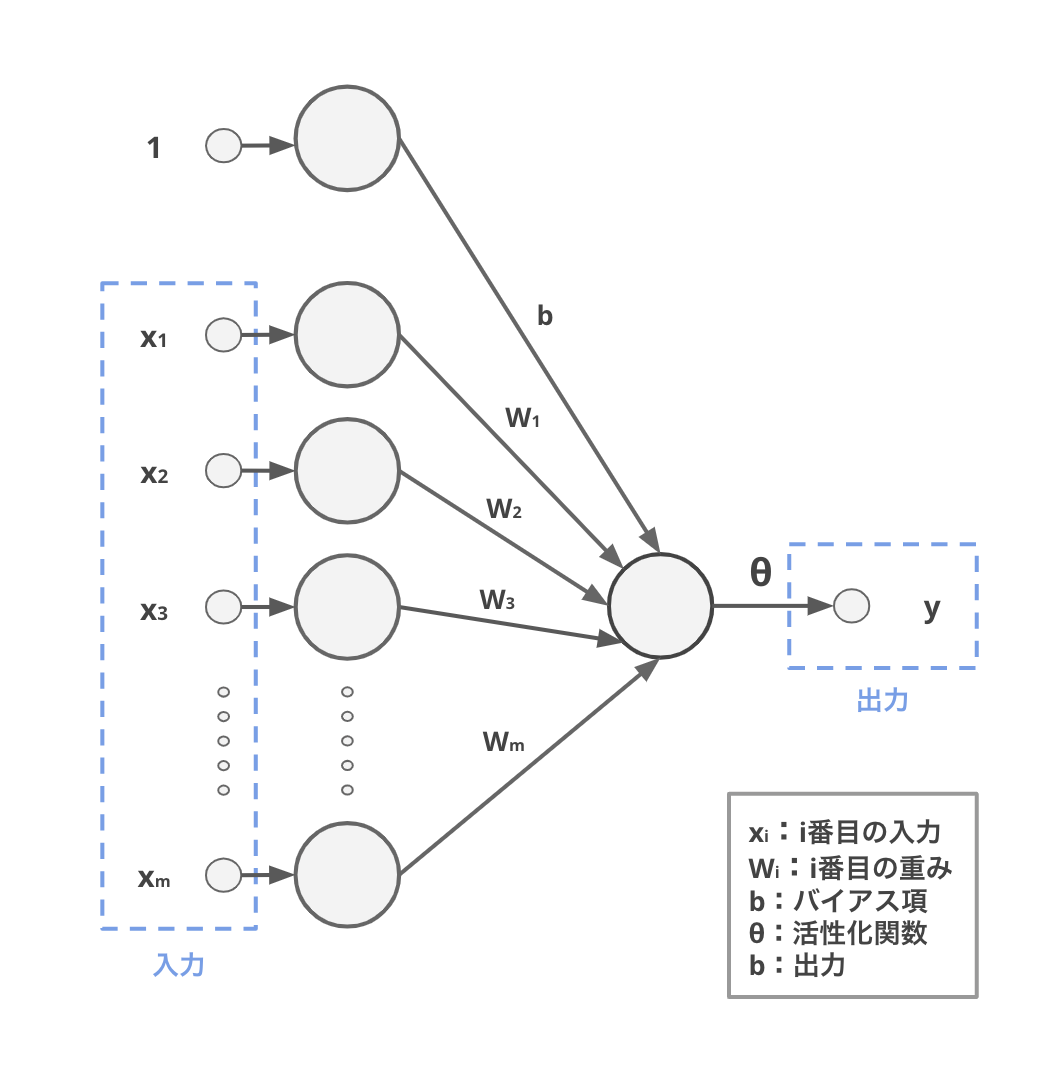
\includegraphics[width=0.6\hsize]{figure/neuron.png}
\caption{人工ニューロン}
\label{fig:neuron}
\end{figure}

MLPにおける人工ニューロンは\prettyref{fig:neuron}のように$m$個の入力$x_i$に対応した重み$w_i$をかけた重み付き和に対して活性関数$\theta$を作用させた出力$y$を返す。つまり、\prettyref{eq:MLP0_0}として定式化される。

\begin{align}
    \label{eq:MLP0_0}
    \boldsymbol{y}=\theta(\sum_{i=1}^{m} W_{i} \times \boldsymbol{x_i})
\end{align}

%ここで改ページ
\clearpage

また、活性化関数としては出力値を調整するために適当な関数が選ばれる。多くの場合は\prettyref{eq:ReLU}のReLU関数や\prettyref{eq:Sigmoid}のSigmoid関数などの非線形関数が用いられる。

\begin{align}
    \label{eq:ReLU}
    \theta_{ReLU}(x)&=max(0,x)\\
    \label{eq:Sigmoid}
    \theta_{Sigmoid}(x)&=\frac{1}{1+e^{-x}}
\end{align}


\subsection{MLPの構造と定式化}

MLPの構成単位は、\prettyref{sec:neuron}の人工ニューロンが複数並んだ層である~(\prettyref{fig:MLP_net0})~。この層の出力$\boldsymbol{y}$は\prettyref{eq:MLP0_0}より\prettyref{eq:MLP0_1}として導出できる。また、$\boldsymbol{x} \mapsto W\boldsymbol{x}+\boldsymbol{b}$はアフィン変換と呼ばれ、$\theta$は活性化関数である。

\begin{figure}[b]
\centering
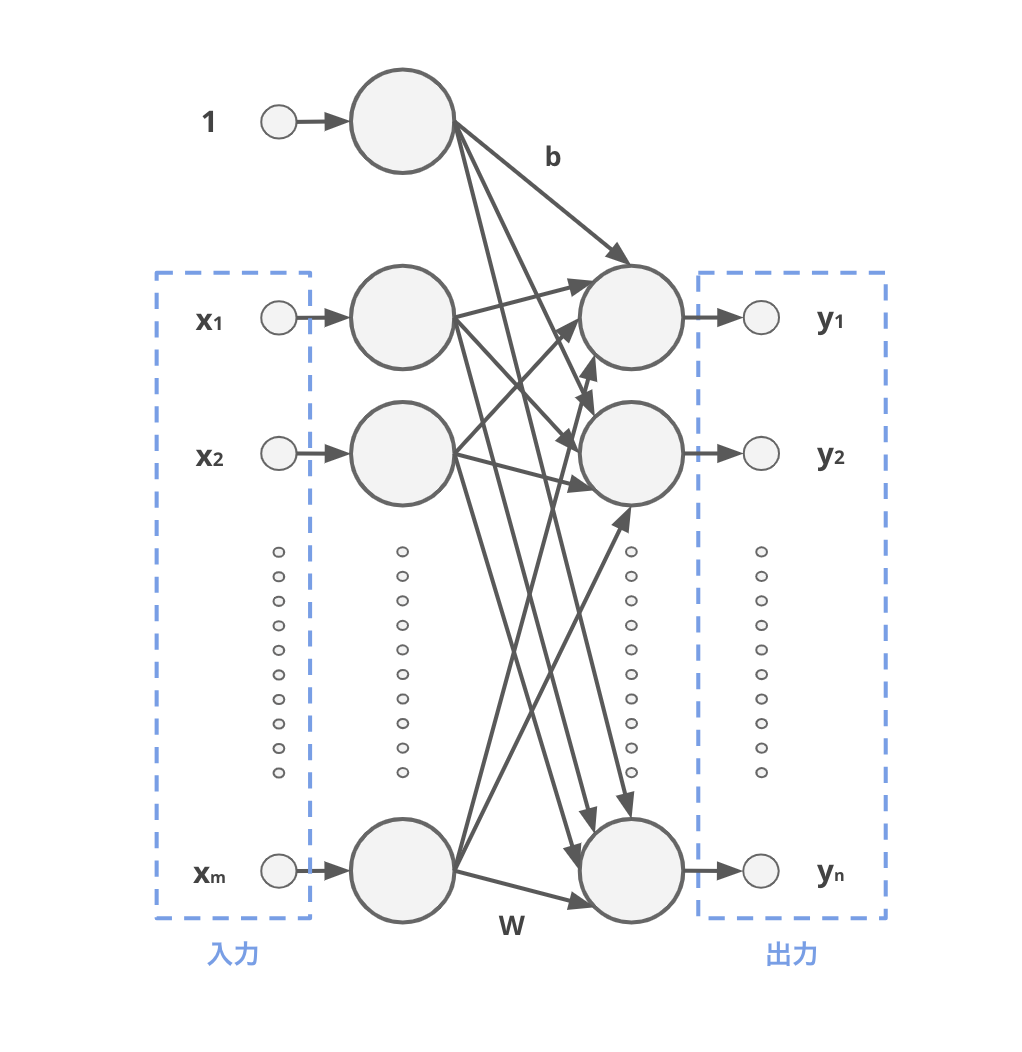
\includegraphics[width=0.6\hsize]{figure/mlp_net0.png}
\caption{MLPの一層}
\label{fig:MLP_net0}
\end{figure}

\begin{align}
    \label{eq:MLP0_1}
    \boldsymbol{y}&=\theta(W\boldsymbol{x}+\boldsymbol{b})
\end{align}

ここで、$\boldsymbol{x}$は層の入力となる実ベクトル、$\boldsymbol{y}$は層の出力となる実ベクトル、$\boldsymbol{b}$は第$i$成分が$i$番目の出力に対応したバイアス項となる実ベクトル、$W$は$(i,j)$成分が$i$番目の人工ニューロンと$i$番目の出力に対応した重みとなる実ベクトル、である。

%ここで改ページ
\clearpage

MLPは、\prettyref{fig:MLP_net0}を一層とした順伝播型の階層構造のニューラルネットワークである~(\prettyref{fig:MLP_net1})~。一層ずつの入力層と出力層、その間の中間層から構成される。層を構成する人工ニューロンの出力は次の層の全ての人工ニューロンに渡されるため、MLPを構成する層を全結合層と呼ぶ。また、$n$を層数とおくことで、MLPは\prettyref{eq:MLP0_2}として定式化される。

\begin{figure}[b]
\centering
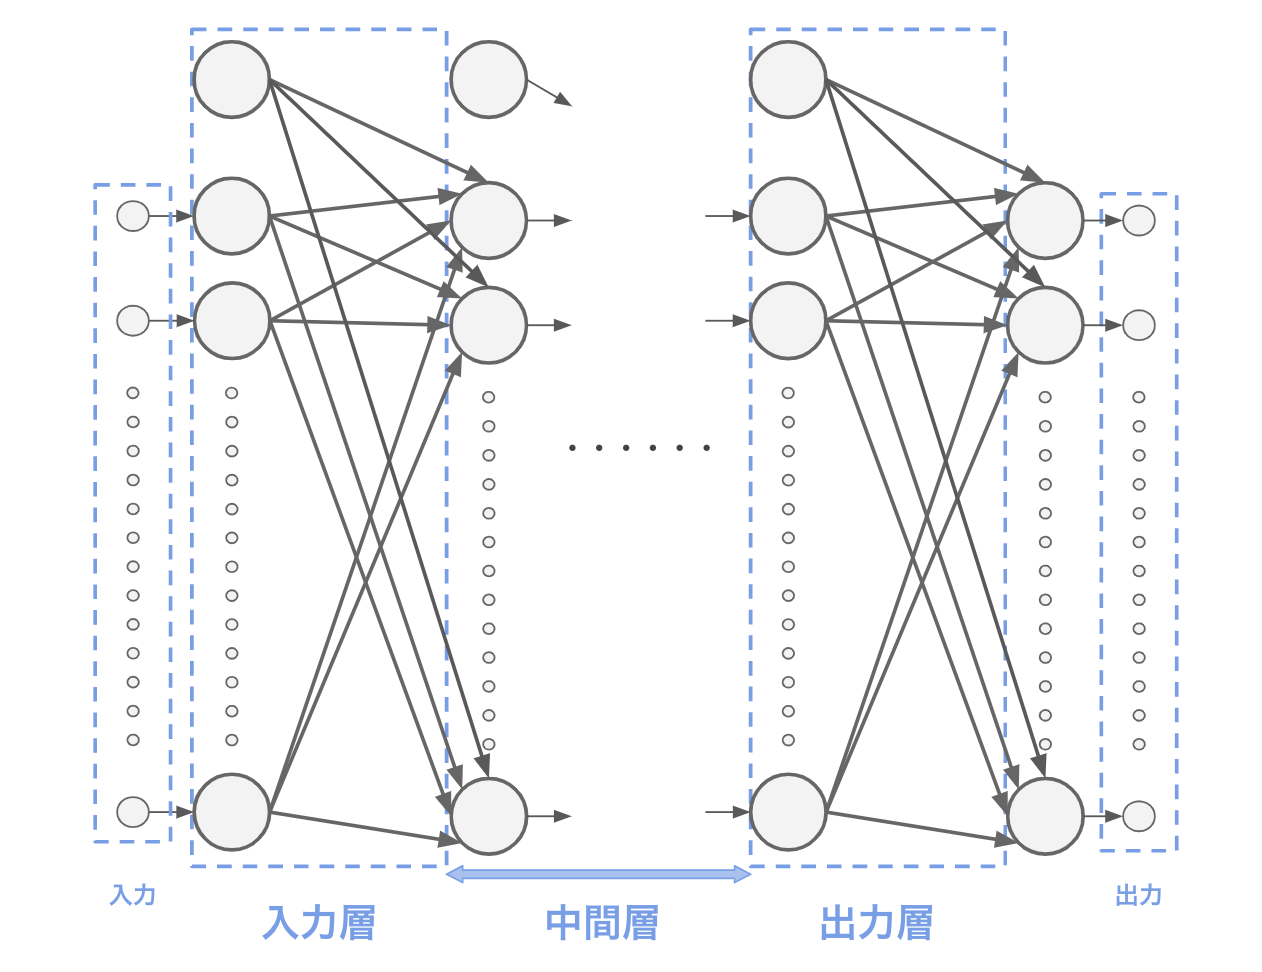
\includegraphics[width=0.8\hsize]{figure/mlp_net1.png}
\caption{MLPのネットワーク}
\label{fig:MLP_net1}
\end{figure}

\begin{align}
    \label{eq:MLP0_2}
    \hat{f}(\boldsymbol{x})&=\theta_{n}(W_{n}(\theta_{n-1}(W_{n-1}\cdots(\theta_{1}(W_{1}\boldsymbol{x}+\boldsymbol{b_{1}}))\cdots+\boldsymbol{b_{n-1}}))+\boldsymbol{b_{n}})
\end{align}

ここで、$\boldsymbol{x}$は実ベクトル、$\theta_{i}$は$i$番目の活性化関数、$W_{i}$は$i$番目の行列、$\boldsymbol{b_{i}}$は$i$番目の実ベクトル、である。


\subsection{MLPの学習}

MLPではバイアス項と層の重みを更新する学習の結果として、任意の$i$で$W_i,\boldsymbol{b_i}$が適切に定まる。また、教師あり学習では損失関数を減少させる方向に学習は進むため、それぞれ\prettyref{eq:MLP2_0}と\prettyref{eq:MLP2_1}にしたがって$W_i,\boldsymbol{b_i}$は更新される~(勾配降下法)~。

\begin{align}
    \label{eq:MLP2_0}
    W _i &\leftarrow W_i - \eta \frac{d L}{dW_i} \\
    \label{eq:MLP2_1}
    \boldsymbol{b _i} &\leftarrow \boldsymbol{b_i} - \eta \frac{d L}{dW_i}
\end{align}

%ここで改ページ
\clearpage

ここで、$L$は損失関数であり、$\eta$は学習率と呼ばれる任意の正の実数である。損失関数としては\prettyref{eq:MLP3}の平均二乗誤差$L_{MSE}$や\prettyref{eq:MLP4}の平均絶対誤差$L_{MAE}$などが用いられる。また、学習率の更新化における最適化アルゴリズムとしてはAdam~\cite{Adam}やStochastic~Gradient~Descent~\cite{SGD}などが用いられる。

\begin{align}
    \label{eq:MLP3}
    L_{MSE}&=\frac{1}{n}\sum _{j} {(\boldsymbol{y_j} - \hat{f}(\boldsymbol{x_j}))^2}\\
    \label{eq:MLP4}
    L_{MAE}&=\frac{1}{n}\sum _{j} {|\boldsymbol{y_j} - \hat{f}(\boldsymbol{x_j})|}
\end{align}

\section{CNN}

CNN~(Convolution~Neural~Network)~は、MLPにおいて全結合層を畳み込み層とプーリング層の繰り返し構造に置換した順伝播型のニューラルネットワークである。

\subsection{CNNの構造}

CNNはネオコグニトロン~\cite{neocognition}を起源に持ち、脳の視覚野の機能を模倣するようなネットワーク構造を持つ。脳の視覚野には主に二つの機能があり、一つ目は刺激の位置により異なったニューロンの活動電位の発生であり、二つ目は受容する情報の特徴の段階的な受容である。畳み込み層では、人工ニューロン間の結合を局所領域に限定することで局所領域の特徴を抽出するため、前者の機能を模倣する。また、プーリング層では、人工ニューロンの結合を局所領域に限定することで局所領域の特徴を集約する。したがって、局所領域の集約によりそれぞれの層で異なったスケールでの情報を受容し、後者の機能を模倣する。

%ここで改ページ
\clearpage

\subsection{畳み込み層}

畳み込み層においては、カーネルと呼ばれるフィルターを一定の間隔~(ストライド)~でスライドさせながらフィルターにより覆われた入力の部分の畳み込み演算を順に行う。畳み込み演算により、カーネルのそれぞれの値を重みとした対応する入力の部分の重み付き和を計算する。また、入力と出力の大きさを変えないために、一般には入力の周りに適当な幅で値を埋める操作を行う~(パディング)~。そして、画像のような二次元データにおいては、畳み込み演算は\prettyref{fig:conv}のように表現することができる。

\begin{figure}[b]
\centering
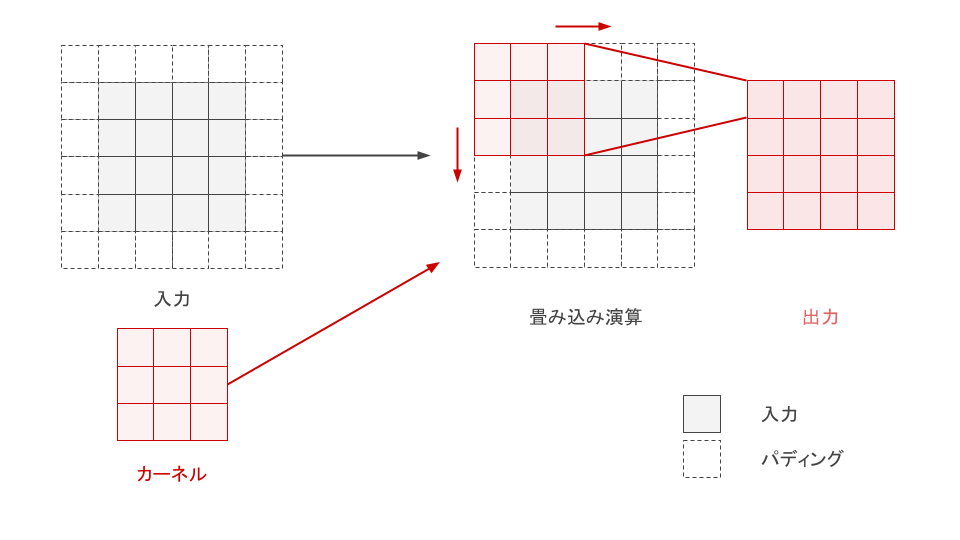
\includegraphics[width=\hsize]{figure/convolution.png}
\caption{畳み込み層}
\label{fig:conv}
\end{figure}

さらに、入力を$I_h \times I_w$の行列、カーネルを$F_h \times F_w$の行列、ストライドを$S_h,S_w$、パディング幅を$P_h,P_w$、出力を$O_h \times O_w$の行列、とすれば、\prettyref{eq:conv}が成り立つ。\prettyref{fig:conv}においては、$I_h=I_w=4,F_h=F_w=3,S_h=S_w=1,P_h=P_w=1$であるため、$O_h=IO_w=4$となる。

\begin{align}
    \label{eq:conv}
    O_{h}&=\frac{I_h+2 P_h-F_{h}}{S_h}+1 \\
    O_{w}&=\frac{I_w+2 P_w-F_{w}}{S_w}+1
\end{align}

また、上記では入力と出力がいずれもチャンネル数が1つの場合を考えたが、実際には複数存在することが多い。したがって、カーネルの数は(入力チャンネル数)$\times$(出力チャンネル数)である。また、それぞれの出力チャンネル数に対し特徴量マップが入力チャンネル数だけ存在するが、これらの和にバイアス項を加えたものが実際の出力となる。

%ここで改ページ
\clearpage

\subsection{プーリング層}

\begin{figure}[b]
\centering
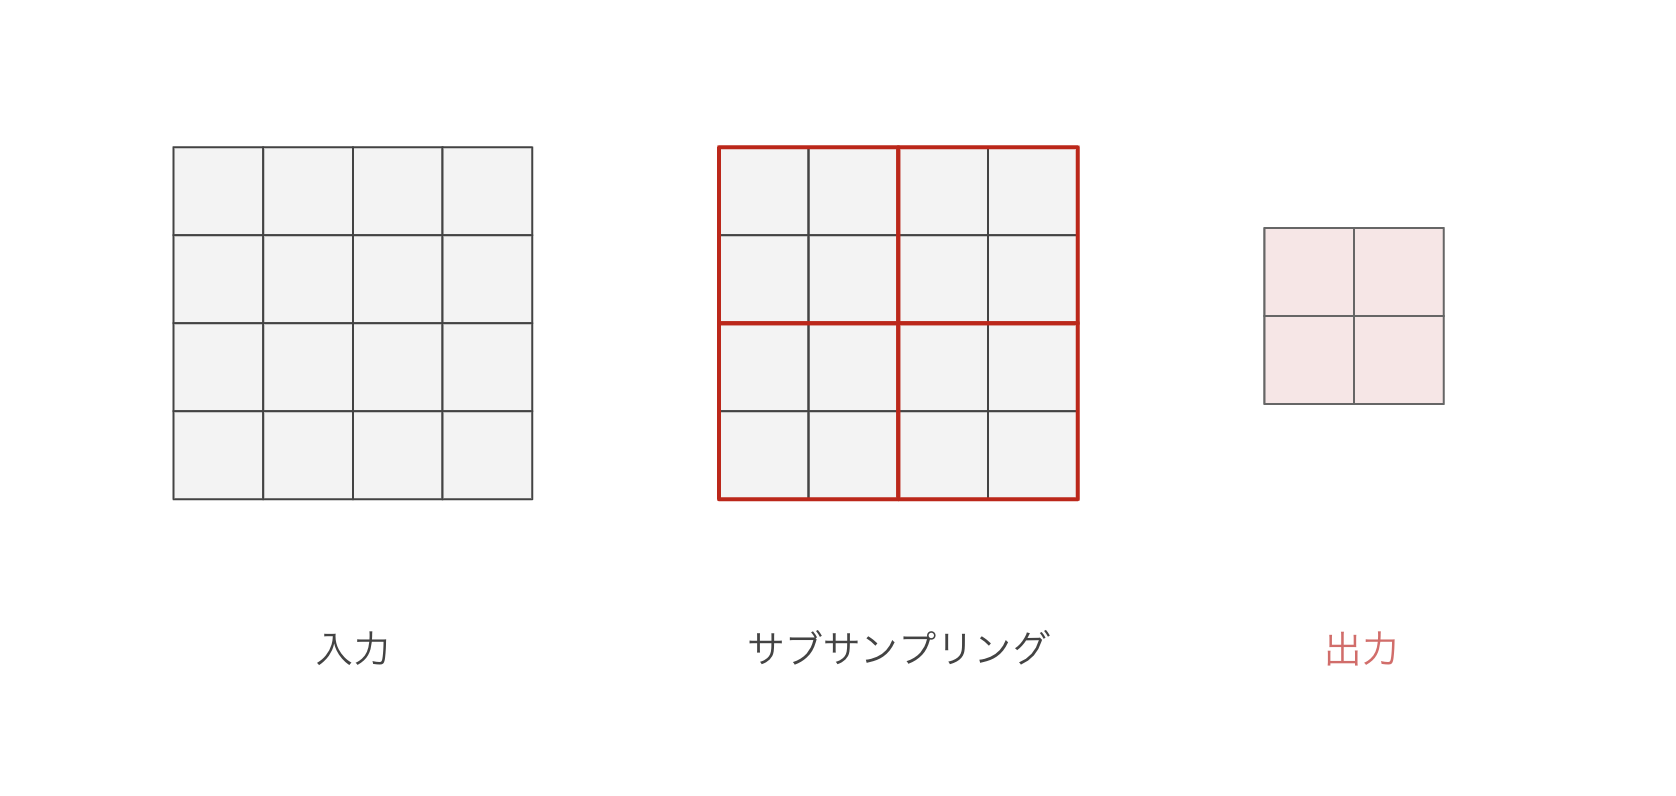
\includegraphics[width=\hsize]{figure/pooling.png}
\caption{プーリング層}
\label{fig:pooling}
\end{figure}

プーリング層においては、入力を局所領域ごとに分解し、領域ごとへの何らかの操作により情報量の圧縮を行う~(サブサンプリング、ダウンサンプリング)~。また、この時の操作で最大値をとる場合はMax~Pooling、平均値をとる場合はAverage~Poolingと呼び、主にこの二つが用いられる。

\subsection{CNNの利点}

CNNにはMLPと比べて主に二つの利点がある~\cite{CNNsurvey}。一つ目は、パラメータ数が減少する点である。全結合層においては入力の数と出力の数の積が層のパラメータ数となるが、畳み込み層においてはカーネルに含まれるパラメータ数のみが層のパラメータ数となるため、通常はパラメータ数が減少する。また、プーリング層においてもサブサンプリングにより特徴量マップのサイズが小さくなるためパラメータ数の減少に寄与する。二つ目は、様々な解像度での特徴を取得できる点である。プーリング層によりサブサンプリングをすることで解像度が低下し、異なるスケールでの隣接する特徴の共起を得ることができると期待される。

%ここで改ページ
\clearpage

\section{GAN}

\begin{figure}[b]
\centering
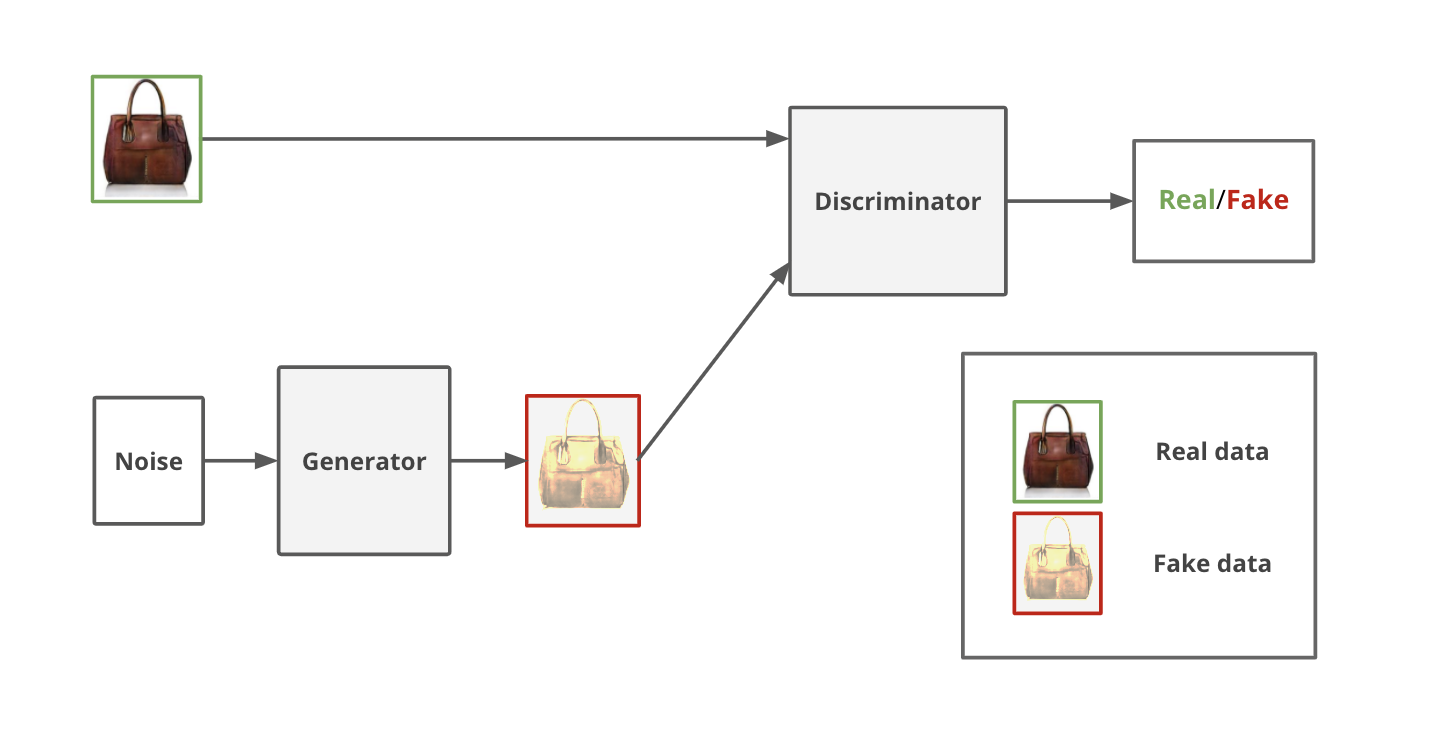
\includegraphics[width=\hsize]{figure/GAN_net.png}
\caption{GANのネットワーク\\
図は~\cite{pix2pix}のFigure~1を用いて作成した。}
\label{fig:GAN_net}
\end{figure}

GAN~(Generative~Adversarial~Networks)~\cite{GAN}はニューラルネットワークの応用例であり、学習データの特徴を持つ擬似的なデータを生成することを目指す手法である。この手法は実在しないアイドルの写真を生成する際などに用いられる~\cite{idol}。また、GANは\prettyref{fig:GAN_net}のように二つのニューラルネットワークで構成され、それぞれのネットワークはDiscriminator~(識別モデル)~とGenerator~(生成モデル)~と呼ばれる。

\subsection{GANの学習}

生成モデルと識別モデルの二つのネットワークはランダムに初期化された後に競合的に学習を進める。まず、識別モデルはデータがFake~data~(生成モデルの出力)~とReal~data~(学習データ)~のどちらであるかを識別できるように学習を進める。そして、生成モデルは識別モデルが学習データであると誤って識別するように、Noise~(ノイズ)~を元に学習データに近いデータを出力する。この二つの学習を交互に繰り返すことで、漸進的に生成モデルが学習データにより近いデータを生成できるようになると期待される。また、ノイズは適当な次元の実ベクトルであり、生成モデルの出力の揺らぎを表現する潜在変数の役割を果たす。

%ここで改ページ
\clearpage

\subsection{GANの定式化}

GANでは、生成モデルの目的関数は\prettyref{eq:GAN_G}、識別モデルの目的関数は\prettyref{eq:GAN_D}として定式化される。

\begin{align}
    \label{eq:GAN_G}
    \argmin _{\theta_G}& \mathbb{E}_{\boldsymbol{z}}[\log (1-D(G(\boldsymbol{z};\theta_G);\theta_D))]\\
    \label{eq:GAN_D}
    \argmax _{\theta_D}& \mathbb{E}_{\boldsymbol{x}}[\log D(\boldsymbol{x};\theta_D)]+\mathbb{E}_{\boldsymbol{z}}[\log (1-D(G(\boldsymbol{z};\theta_G);\theta_D))]
\end{align}


ここで、$\boldsymbol{x}$は学習データ、$\boldsymbol{z}$は生成モデルへの入力のノイズ、$G(\boldsymbol{z};\theta_G)$はノイズ$\boldsymbol{z}$を入力とする生成モデル、$D(\cdot;\theta_D)$は識別モデル、$\theta_G$は生成モデル$G$のパラメータ、$\theta_D$は識別モデル$D$のパラメータ、である。

\section{Pix2pix}

Pix2pix~\cite{pix2pix}は、\prettyref{fig:pix2pix_net}のようにネットワークの入力に変換元の画像を~Condition~(条件)~として与えることで画像の変換を行うGANである。特定の条件をネットワークの入力に与えるGANとしてはConditional~GAN~(CGAN)~\cite{CGAN}が初めて考案されたが、Pix2pixは与えられた条件画像の構造を維持したまま変換するという点でCGANとは異なる。具体的には、\prettyref{fig:pix2pix_img}のように線画から写真への変換や白黒画像からカラー画像への変換を行うことができる。

\begin{figure}[b]
\centering
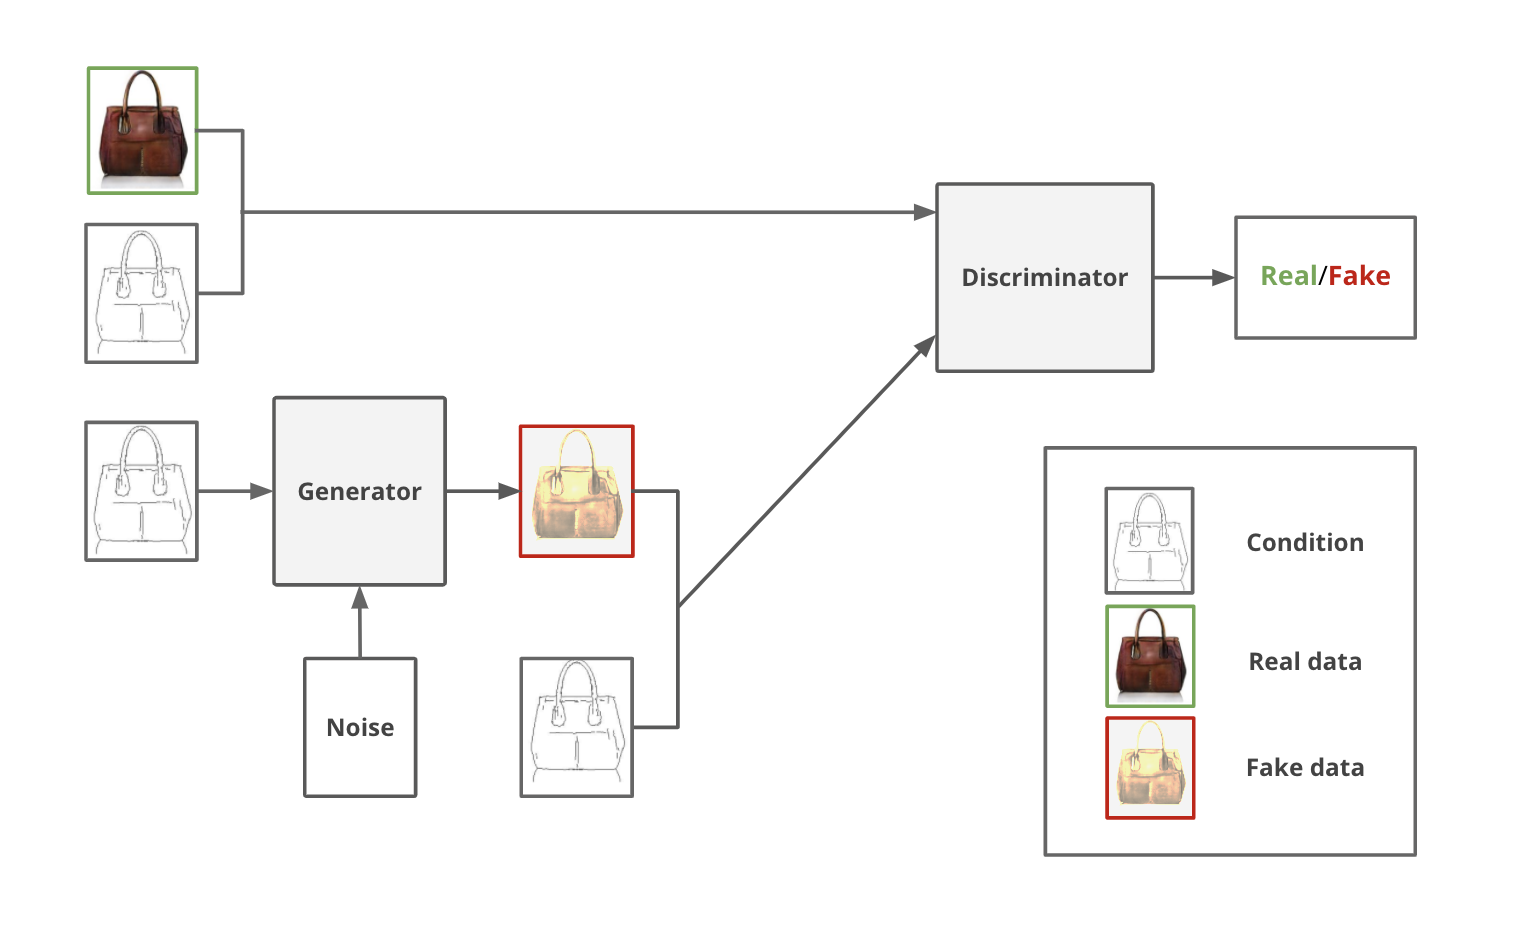
\includegraphics[width=0.9\hsize]{figure/pix2pix_net.png}
\caption{Pix2pixのネットワーク\\
図は~\cite{pix2pix}のFigure~1を用いて作成した。}
\label{fig:pix2pix_net}
\end{figure}

%ここで改ページ
\clearpage

\begin{figure}[t]
\centering
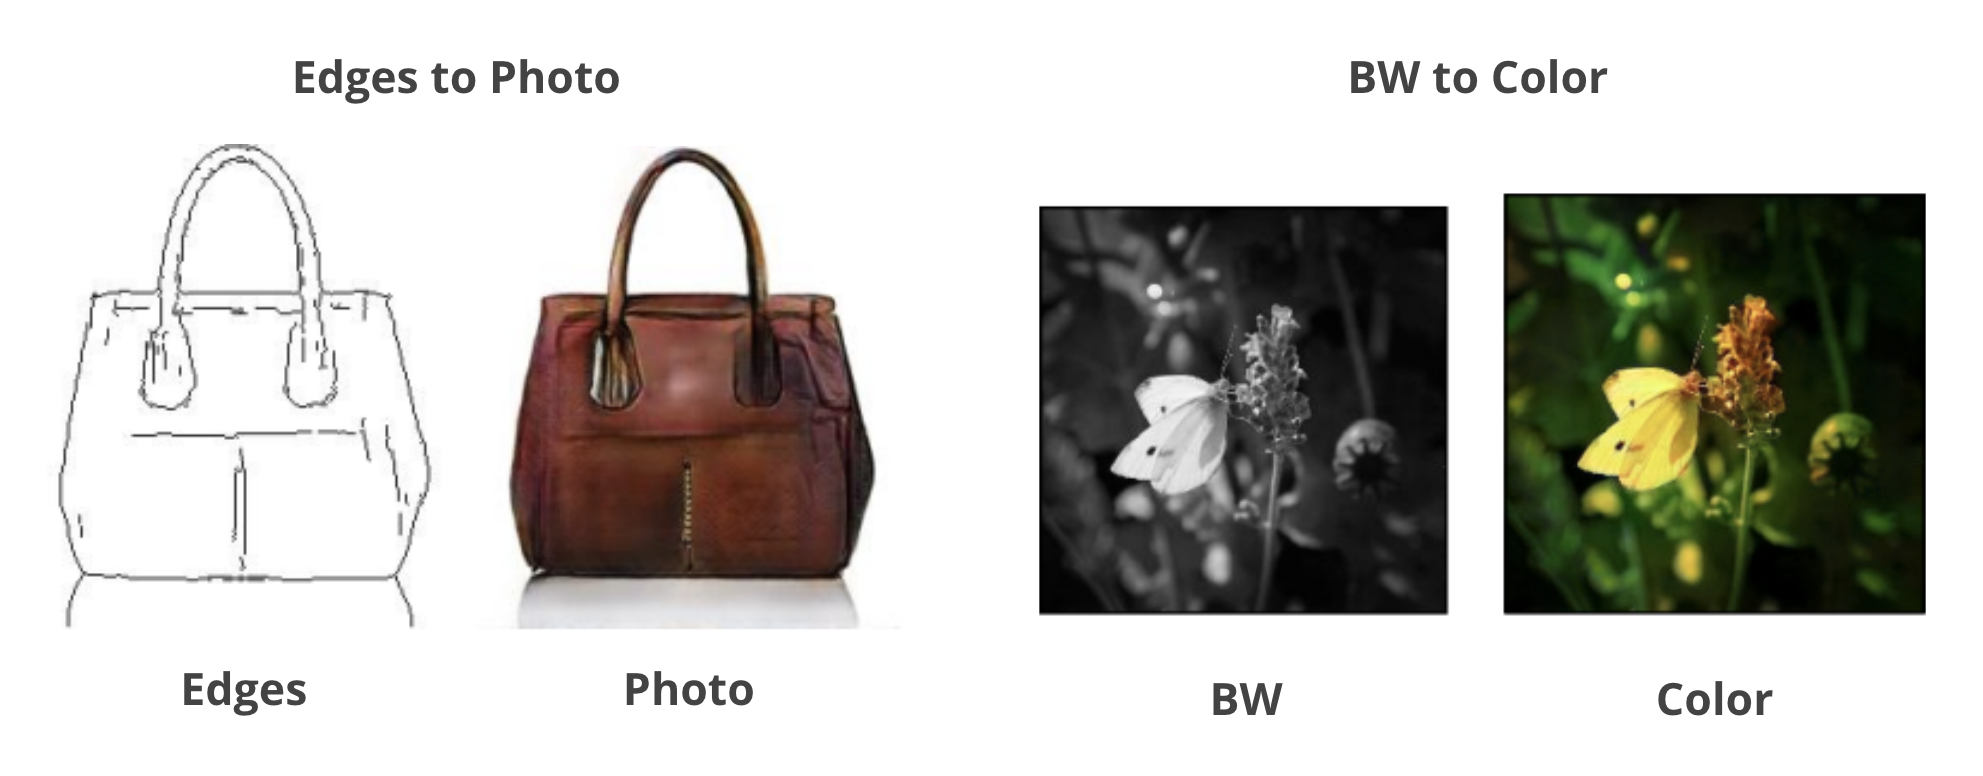
\includegraphics[width=\hsize]{figure/pix2pix_img.png}
\caption{Pix2pixのスタイル変換の例\\
図は~\cite{pix2pix}のFigure~1を用いて作成した。}
\label{fig:pix2pix_img}
\end{figure}

\subsection{Pix2pixの定式化}

そして、Pix2pixにおいては、生成モデルの目的関数は\prettyref{eq:pix2pix_G}、識別モデルの目的関数は\prettyref{eq:pix2pix_D}として定式化される。

\begin{align}
    \label{eq:pix2pix_G}
    \argmin _{\theta_G}& \mathbb{E}_{\boldsymbol{y}, \boldsymbol{z}}[\log (1-D(\boldsymbol{y}, G(\boldsymbol{y}, \boldsymbol{z}; \theta_G); \theta_D))]+\mathbb{E}_{\boldsymbol{x}, \boldsymbol{y}, \boldsymbol{z}}[\|\boldsymbol{x}-G(\boldsymbol{y}, \boldsymbol{z}; \theta_G)\|_{1}]\\
    \label{eq:pix2pix_D}
    \argmax _{\theta_D}& \mathbb{E}_{\boldsymbol{x}, \boldsymbol{y}}[\log D(\boldsymbol{x}, \boldsymbol{y}; \theta_D)]+\mathbb{E}_{\boldsymbol{y}, \boldsymbol{z}}[\log (1-D(\boldsymbol{y}, G(\boldsymbol{y}, \boldsymbol{z}; \theta_G); \theta_D))]
\end{align}

ここで、$\boldsymbol{x}$は変換先の学習データ、$\boldsymbol{y}$は変換元の学習データ、$\boldsymbol{z}$は生成モデルへの入力のノイズ、$G(\boldsymbol{y},\boldsymbol{z};\theta_G)$は$\boldsymbol{y}$を条件としノイズ$\boldsymbol{z}$を入力とする生成モデル、$D(\boldsymbol{y},\cdot;\theta_D)$は$\boldsymbol{y}$を条件とする識別モデル、$\theta_G$は生成モデル$G$のパラメータ、$\theta_D$は識別モデル$D$のパラメータ、である。

\subsection{Pix2pixの生成モデル}

Pix2pixの生成モデルには、\prettyref{fig:u-net}のようにEncoder-Decoder型のネットワークが用いられる。ただし、変換元の画像と返還後の画像で共通する基本構造であるピクセルの対応関係を維持するために、スキップコネクションが用いられる。このスキップコネクションはU-net~\cite{u-net}で用いられたものと同様の働きをする。具体的には、エンコード前の特徴量マップをデコード時にも利用しており、この特徴量マップによりピクセルの対応関係が維持されると期待される。

また、ノイズとしては実ベクトルではなくDropout~\cite{Dropout}が用いられる。Dropoutとは、ニューラルネットワークの重みの更新の際にランダムにいくつかの重みを0として無視する手法のことである。

%ここで改ページ
\clearpage

\begin{figure}[t]
\centering
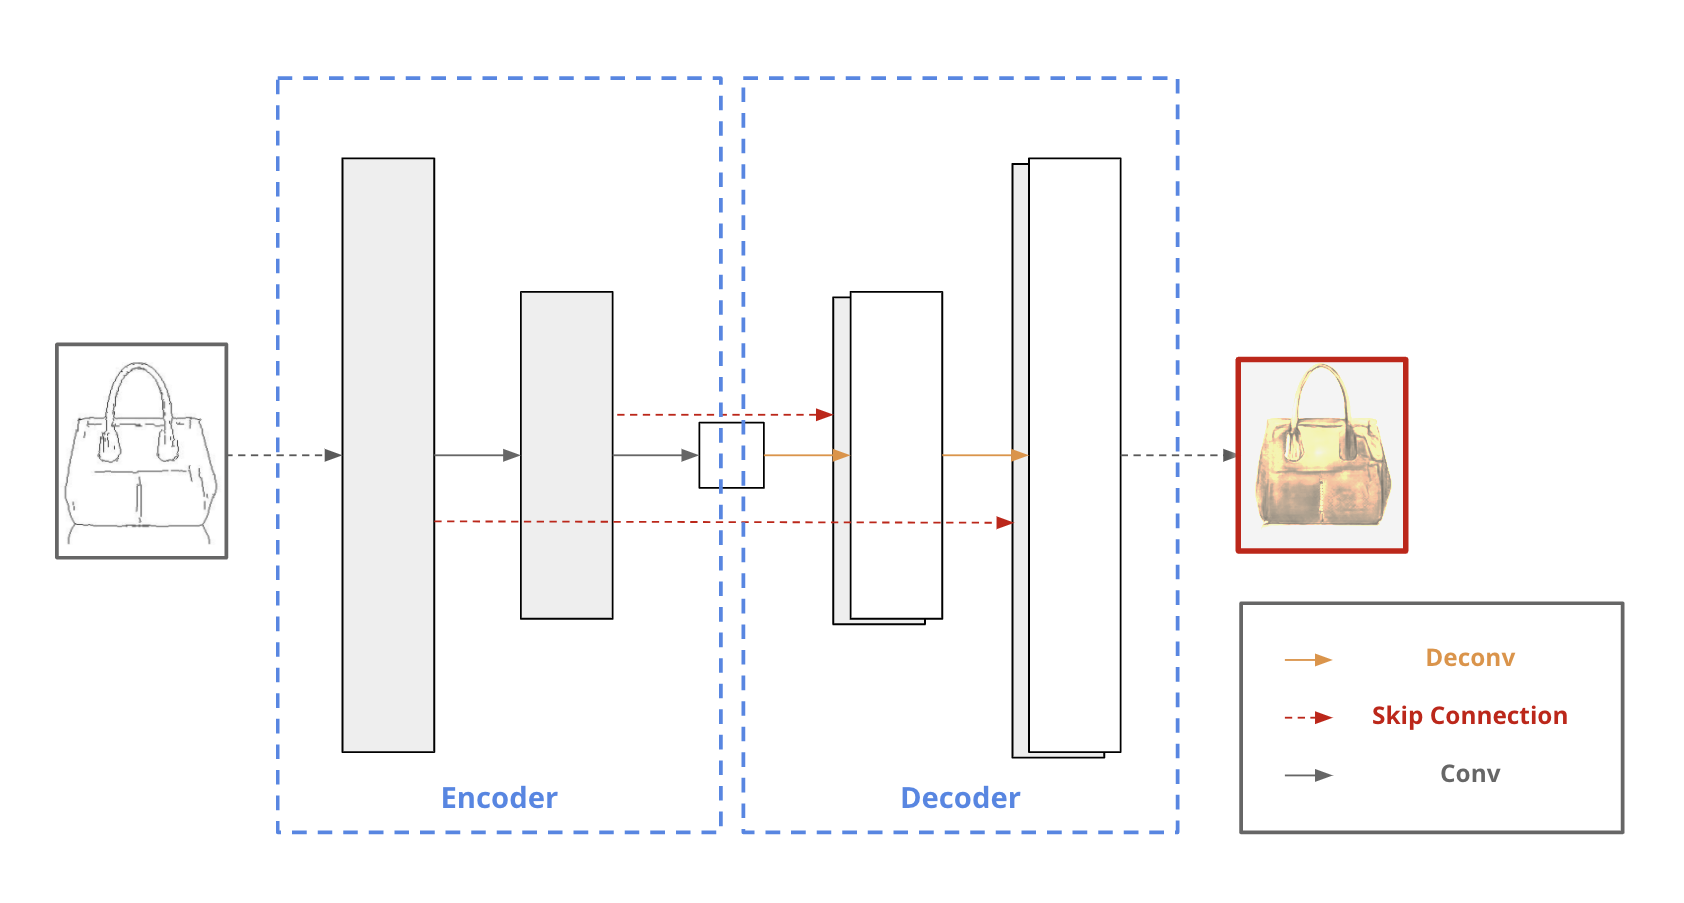
\includegraphics[width=0.8\hsize]{figure/u-net.png}
\caption{生成モデルのネットワーク\\
図は~\cite{pix2pix}のFigure~1とFigure~3を用いて作成した。}
\label{fig:u-net}
\end{figure}

\subsection{Pix2pixの識別モデル}

\begin{figure}[b]
\centering
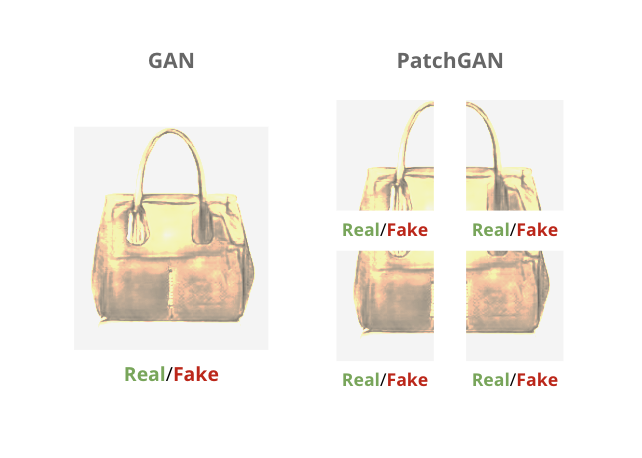
\includegraphics[width=0.6\hsize]{figure/patchgan.png}
\caption{通常のGANとPatchGANの比較\\
図は~\cite{pix2pix}のFigure~1を用いて作成した。}
\label{fig:patchgan}
\end{figure}

Pix2pixの識別モデルには、PatchGANという手法が用いられる。PatchGANは\prettyref{fig:patchgan}のように画像全体ではなくパッチと呼ばれる局所領域ごとに真偽を求めて平均を出力とする。これにより、局所的な識別精度が高まることが期待される。